
\begin{enumerate}[\Large \bfseries 1.]


\begin{comment}
%----------molde.
\item 

\begin{enumerate}[\bfseries a)]
    
    %----------a)
    \item \textbf{Análisis del problema.}\\

    %----------b)
    \item \textbf{Diagrama de flujo.}\\
	\begin{center}
	    %\includegraphics[scale=.37]{imagenes}
	\end{center}

    %----------c)
    \item \textbf{Prueba de escritorio.}\\
	\begin{center}
	    \begin{tabular}{c|c}
	    \end{tabular}
	\end{center}
	\vspace{4cm}
    
    %----------d)
    \item \textbf{Código fuente.}\\ 
	
	%\lstinputlisting[language=Python]{python}
	\vspace{3cm}
    
    %----------e)
    \item \textbf{Prueba de la ejecución del programa}.\\
	\begin{center}
	    %\includegraphics[scale=.5]{imagenes}
	\end{center}

\end{enumerate}

\newpage
\end{comment}


%-------------------- funciones --------------------

%----------extra 1.
\item Geometría: área de un pentágono. El área de un pentágono se puede calcular utilizando la siguiente fórmula: 
    $$area = \dfrac{5\cdot lado^2}{4\cdot \tan\left(\dfrac{\pi}{5}\right)}$$
    Escriba un método que devuelva el área de un pentágono.\\\\

\begin{enumerate}[\bfseries a)]
    
    %----------d)
    \item \textbf{Código fuente.}\\ 
	
	\lstinputlisting[language=Python]{python/extras/geometria.py}
	\vspace{1cm}
    
    %----------e)
    \item \textbf{Prueba de la ejecución del programa}.\\
	\begin{center}
	    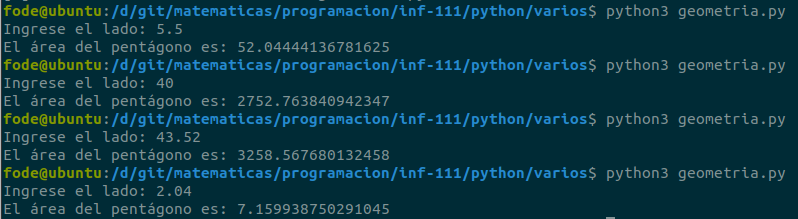
\includegraphics[scale=.5]{imagenes/extras/geometria.png}
	\end{center}

\end{enumerate}

\newpage
\end{enumerate}
